\documentclass[8pt]{article}
\usepackage{tikz}
\usetikzlibrary{bayesnet}
\usepackage{amsmath}
\usetikzlibrary{arrows}

\begin{document}

\begin{figure*}[ht]
\centering
\resizebox{1\textwidth}{!}{
    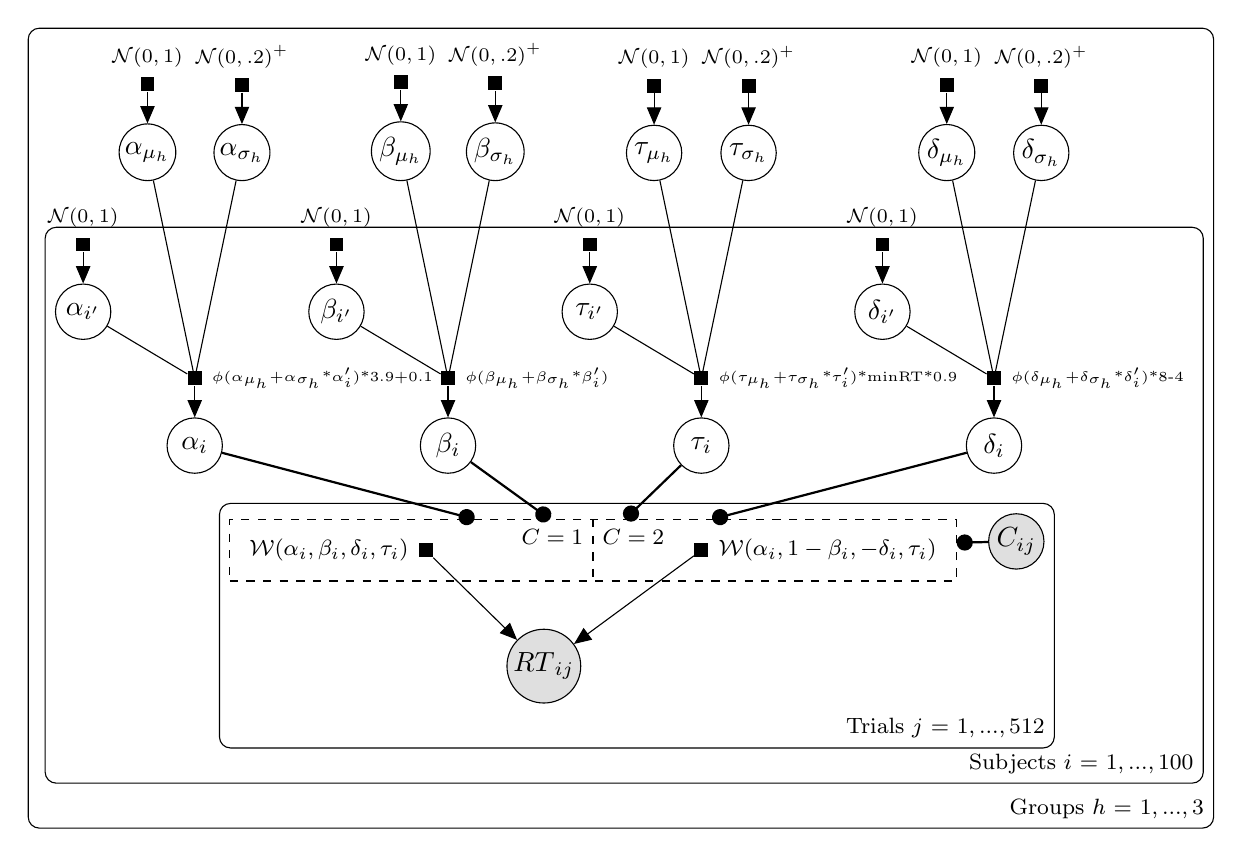
\begin{tikzpicture}

        %add choice and RT nodes
        \node[obs](RT) {$\var{RT}_{ij}$}; %RT grey node
        \node[obs, above=of RT,xshift= 6cm, yshift= -0.25cm] (C) {$\var{C}_{ij}$}; %choice ("C") grey node

        %tau
        \node[latent, above=of C, xshift= -4cm,yshift=-0.5cm] (tau_i) {$\tau_{i}$};
        \node[latent, above=of tau_i, xshift= -0.6cm,yshift=2cm] (tau_mu) {$\tau_{\mu_h}$};
        \node[latent, above=of tau_i, xshift= 0.6cm,yshift=2cm] (tau_sigma) {$\tau_{\sigma_h}$};
        \node[latent, left=of tau_i, xshift=0.3cm,yshift=1.7cm] (tau_iprime) {$\tau_{i'}$};
        \factor[above=of tau_i] {tau_i-f} {right:\tiny $\phi(\tau_{\mu_h}$+$\tau_{\sigma_h}$*$\tau_i')$*minRT*0.9} {tau_mu, tau_sigma,tau_iprime} {tau_i} 
        \factor[above=of tau_mu] {tau_mu-f} {above:\scriptsize$\mathcal{N}(0,1)$} {} {tau_mu}    
        \factor[above=of tau_sigma] {tau_sigma-f} {above:\scriptsize$\mathcal{N}(0,.2)^+$} {} {tau_sigma} 
        
        %delta
        \node[latent, right=of tau_i, xshift= 2cm] (delta_i) {$\delta_i$};
        \node[latent, above=of delta_i, xshift= -0.6cm,yshift=2cm] (delta_mu) {$\delta_{\mu_h}$};
        \node[latent, above=of delta_i, xshift= 0.6cm,yshift=2cm] (delta_sigma) {$\delta_{\sigma_h}$};
        \node[latent, left=of delta_i, xshift=0.3cm,yshift=1.7cm] (delta_iprime) {$\delta_{i'}$};
        \factor[above=of delta_i] {delta_i-f} {right:\tiny $\phi(\delta_{\mu_h}$+$\delta_{\sigma_h}$*$\delta_i')$*8-4} {delta_mu, delta_sigma,delta_iprime} {delta_i}         
        \factor[above=of delta_mu] {delta_mu-f} {above:\scriptsize$\mathcal{N}(0,1)$} {} {delta_mu}     
        \factor[above=of delta_sigma] {delta_sigma-f} {above:\scriptsize$\mathcal{N}(0,.2)^+$} {} {delta_sigma} 

        %beta
        \node[latent, left=of tau_i, xshift= -1.5cm] (beta_i) {$\beta_i$};
        \node[latent, above=of beta_i, xshift= -0.6cm,yshift=2cm] (beta_mu) {$\beta_{\mu_h}$};
        \node[latent, above=of beta_i, xshift= 0.6cm,yshift=2cm] (beta_sigma) {$\beta_{\sigma_h}$};
        \node[latent, left=of beta_i, xshift=0.3cm,yshift=1.7cm] (beta_iprime) {$\beta_{i'}$};
        \factor[above=of beta_i] {beta_i-f} {right:\tiny $\phi(\beta_{\mu_h}$+$\beta_{\sigma_h}$*$\beta_i')$} {beta_mu, beta_sigma,beta_iprime} {beta_i}
        \factor[above=of beta_mu] {beta_mu-f} {above:\scriptsize$\mathcal{N}(0,1)$} {} {beta_mu}          
        \factor[above=of beta_sigma] {beta_sigma-f} {above:\scriptsize$\mathcal{N}(0,.2)^+$} {} {beta_sigma} 

        %alpha
        \node[latent, left=of beta_i, xshift= -1.5cm] (alpha_i) {$\alpha_i$};
        \node[latent, above=of alpha_i, xshift= -0.6cm,yshift=2cm] (alpha_mu) {$\alpha_{\mu_h}$};
        \node[latent, above=of alpha_i, xshift= 0.6cm,yshift=2cm] (alpha_sigma) {$\alpha_{\sigma_h}$};
        \node[latent, left=of alpha_i, xshift=0.3cm,yshift=1.7cm] (alpha_iprime) {$\alpha_{i'}$};
        \factor[above=of alpha_i] {alpha_i-f} {right:\tiny $\phi(\alpha_{\mu_h}$+$\alpha_{\sigma_h}$*$\alpha_i')$*3.9+0.1} {alpha_mu, alpha_sigma,alpha_iprime} {alpha_i}  
        \factor[above=of alpha_mu] {alpha_mu-f} {above:\scriptsize$\mathcal{N}(0,1)$} {} {alpha_mu}          
        \factor[above=of alpha_sigma] {alpha_sigma-f} {above:\scriptsize$\mathcal{N}(0,.2)^+$} {} {alpha_sigma}       
        %add priors on subject level parameters
        \factor[above=of delta_iprime] {delta_iprime-f} {above:\scriptsize$\mathcal{N}(0,1)$} {} {delta_iprime}
        \factor[above=of tau_iprime] {tau_iprime-f} {above:\scriptsize$\mathcal{N}(0,1)$} {} {tau_iprime}
        \factor[above=of beta_iprime] {beta_iprime-f} {above:\scriptsize$\mathcal{N}(0,1)$} {} {beta_iprime}
        \factor[above=of alpha_iprime] {alpha_iprime-f} {above:\scriptsize$\mathcal{N}(0,1)$} {} {alpha_iprime}

        %wiener distribution
        \factor[above=of RT, xshift= 2cm, yshift= 0.5cm] {C_2} {right:$\mathcal{W}(\alpha_i, 1-\beta_i, -\delta_i, \tau_i)$} {} {RT}; 
        \factor[above=of RT, xshift= -1.5cm, yshift= 0.5cm] {C_1} {left:$\mathcal{W}(\alpha_i, \beta_i, \delta_i, \tau_i)$} {} {RT};
                  
        \vgate {criterion} %gate
            {(C_1)(C_1-caption)} {$C=1$} %yes
            {(C_2)(C_2-caption)} {$C=2$} %no
            {C,delta_i, tau_i, beta_i, alpha_i} ; %input

        %for all trials j in 1:total trials (L)
        \plate{trials} {(criterion) (RT) (C)
        } {Trials $j$ = $1,...,512$}
        
        %for all subjects i in 1:total subjects (M)
        \plate{subjects} {(criterion) (RT) (C) (trials-caption) 
        (alpha_i-f) (alpha_i)
        (alpha_iprime-f) (alpha_iprime)
        (beta_i-f) (beta_i)
        (delta_i-f) (delta_i-f-caption)
        (tau_i-f-caption) (tau_i)
        } {Subjects $i$ = $1,...,100$}

        %for all groups h in 1:total groups (N)
        \plate{groups} {(criterion) (RT) (C) (subjects) 
        (alpha_i-f-caption) (alpha_i)
        (alpha_iprime-f-caption) (alpha_iprime)
        (beta_i-f-caption) (beta_i)
        (delta_i-f-caption) (delta_i)
        (tau_i-f-caption) (tau_i)
        (alpha_mu-f-caption) (alpha_mu)
        } {Groups $h$ = $1,...,3$}
    
    \end{tikzpicture}
}
\end{figure*}

\end{document}
%note - compiled with pdflatex